\documentclass[12pt, dvipsnames]{report}

\usepackage{amsmath}
\usepackage{algorithm}
%\usepackage{algorithmic}
\usepackage[noend]{algpseudocode}

\usepackage{amsmath}
\usepackage{amssymb}
\usepackage{amsthm}
\usepackage{amsopn}

\usepackage{kpfonts}

\usepackage{graphicx}

% Probably don't need this on notes anymore
%\usepackage{kbordermatrix}

% Standard tool for drawing diagrams.
\usepackage{tikz}
\usepackage{tkz-berge}
\usepackage{tikz-cd}
\usepackage{tkz-graph}

\usepackage{comment}

%
\usepackage{multicol}

%
\usepackage{framed}

%
\usepackage{mathtools}

%
\usepackage{float}

%
\usepackage{subfig}

%
\usepackage{wrapfig}

%
\let\savewideparen\wideparen
\let\wideparen\relax
\usepackage{mathabx}
\let\wideparen\savewideparen

% Used for generating `enlightening quotes'
\usepackage{epigraph}

% Forget what this is used for :P
\usepackage[utf8]{inputenc}

% Used for generating quotes.
\usepackage{csquotes}

% Allows what to generate links inside
% generated pdf files
\usepackage{hyperref}

% Allows one to customize theorem
% environments in mathematical proofs.
\usepackage{thmtools}

% Gives access to a proof
\usepackage{lplfitch}

% I forget what this is for.
\usepackage{accents}

% A package for drawing simple trees,
% as a substitute for unnesacary TIKZ code
\usepackage{qtree}

% Enables sequent calculus proofs
\usepackage{ebproof}

% For braket notation
\usepackage{braket}

% To change line spacing when using mathematical notations which require some height!
\usepackage{setspace}

%\usepackage[dvipsnames]{xcolor}

\usepackage{float}

% For block commenting
\usepackage{comment}




\setlength\epigraphwidth{8cm}

\usetikzlibrary{arrows, petri, topaths, decorations.markings}

% So you can do calculations in coordinate specifications
\usetikzlibrary{calc}
\usetikzlibrary{angles}

\theoremstyle{plain}
\newtheorem{theorem}{Theorem}[chapter]
\newtheorem{axiom}{Axiom}
\newtheorem{lemma}[theorem]{Lemma}
\newtheorem{corollary}[theorem]{Corollary}
\newtheorem{prop}[theorem]{Proposition}
\newtheorem{exercise}{Exercise}[chapter]
\newtheorem{fact}{Fact}[chapter]

\newtheorem*{example}{Example}
\newtheorem*{proof*}{Proof}

\theoremstyle{remark}
\newtheorem*{exposition}{Exposition}
\newtheorem*{remark}{Remark}
\newtheorem*{remarks}{Remarks}

\theoremstyle{definition}
\newtheorem*{defi}{Definition}

\usepackage{hyperref}
\hypersetup{
    colorlinks = true,
    linkcolor = black,
}

\usepackage{textgreek}

\makeatletter
\renewcommand*\env@matrix[1][*\c@MaxMatrixCols c]{%
  \hskip -\arraycolsep
  \let\@ifnextchar\new@ifnextchar
  \array{#1}}
\makeatother

\renewcommand*\contentsname{\hfill Table Of Contents \hfill}

\newcommand{\optionalsection}[1]{\section[* #1]{(Important) #1}}
\newcommand{\deriv}[3]{\left. \frac{\partial #1}{\partial #2} \right|_{#3}} % partial derivative involving numerator and denominator.
\newcommand{\lcm}{\operatorname{lcm}}
\newcommand{\im}{\operatorname{im}}
\newcommand{\bint}{\mathbf{Z}}
\newcommand{\gen}[1]{\langle #1 \rangle}

\newcommand{\End}{\operatorname{End}}
\newcommand{\Mor}{\operatorname{Mor}}
\newcommand{\Id}{\operatorname{id}}
\newcommand{\visspace}{\text{\textvisiblespace}}
\newcommand{\Gal}{\text{Gal}}

\newcommand{\xor}{\oplus}
\newcommand{\ft}{\wedge}
\newcommand{\ift}{\vee}

\newcommand{\prob}{\mathbf{P}}
\newcommand{\expect}{\mathbf{E}}
\DeclareMathOperator{\Var}{\mathbf{V}}
\newcommand{\Ber}{\text{Ber}}
\newcommand{\Bin}{\text{Bin}}

%\newcommand{\widecheck}[1]{{#1}^{\ft}}

\DeclareMathOperator{\diam}{\text{diam}}

\DeclareMathOperator{\QQ}{\mathbf{Q}}
\DeclareMathOperator{\ZZ}{\mathbf{Z}}
\DeclareMathOperator{\RR}{\mathbf{R}}
\DeclareMathOperator{\HH}{\mathbf{H}}
\DeclareMathOperator{\CC}{\mathbf{C}}
\DeclareMathOperator{\AB}{\mathbf{A}}
\DeclareMathOperator{\PP}{\mathbf{P}}
\DeclareMathOperator{\MM}{\mathbf{M}}
\DeclareMathOperator{\VV}{\mathbf{V}}
\DeclareMathOperator{\TT}{\mathbf{T}}
\DeclareMathOperator{\LL}{\mathcal{L}}
\DeclareMathOperator{\EE}{\mathbf{E}}
\DeclareMathOperator{\NN}{\mathbf{N}}
\DeclareMathOperator{\DQ}{\mathcal{Q}}
\DeclareMathOperator{\IA}{\mathfrak{a}}
\DeclareMathOperator{\IB}{\mathfrak{b}}
\DeclareMathOperator{\IC}{\mathfrak{c}}
\DeclareMathOperator{\IP}{\mathfrak{p}}
\DeclareMathOperator{\IQ}{\mathfrak{q}}
\DeclareMathOperator{\IM}{\mathfrak{m}}
\DeclareMathOperator{\IN}{\mathfrak{n}}
\DeclareMathOperator{\IK}{\mathfrak{k}}
\DeclareMathOperator{\ord}{\text{ord}}
\DeclareMathOperator{\Ker}{\textsf{Ker}}
\DeclareMathOperator{\Coker}{\textsf{Coker}}
\DeclareMathOperator{\emphcoker}{\emph{coker}}
\DeclareMathOperator{\pp}{\partial}
\DeclareMathOperator{\tr}{\text{tr}}

\DeclareMathOperator{\supp}{\text{supp}}

\DeclareMathOperator{\codim}{\text{codim}}

\DeclareMathOperator{\minkdim}{\dim_{\mathbf{M}}}
\DeclareMathOperator{\hausdim}{\dim_{\mathbf{H}}}
\DeclareMathOperator{\lowminkdim}{\underline{\dim}_{\mathbf{M}}}
\DeclareMathOperator{\upminkdim}{\overline{\dim}_{\mathbf{M}}}
\DeclareMathOperator{\lhdim}{\underline{\dim}_{\mathbf{M}}}
\DeclareMathOperator{\lmbdim}{\underline{\dim}_{\mathbf{MB}}}
\DeclareMathOperator{\packdim}{\text{dim}_{\mathbf{P}}}
\DeclareMathOperator{\fordim}{\dim_{\mathbf{F}}}

\DeclareMathOperator*{\argmax}{arg\,max}
\DeclareMathOperator*{\argmin}{arg\,min}

\DeclareMathOperator{\ssm}{\smallsetminus}

\title{Complex Analysis}
\author{Jacob Denson}

\begin{document}

\pagenumbering{gobble}
\maketitle
\tableofcontents
\pagenumbering{arabic}

\chapter{Introduction}

\section{The Complex Numbers}

In your mathematical career, you must have heard rumours of the exotic `complex numbers'. Like a creature from a far land, these numbers defy the natural properties of $\mathbf{R}$. We begin by categorizing what exactly these numbers are. There are many ways, and they all offer their own intuitions. First, a definition favouring numerical intuition.

\begin{definition}
    The complex number system $\mathbf{C}$ is obtained as the field extension of $\mathbf{R}$, adding a number $i$ for which $i^2 = -1$. Formally, $\mathbf{C}$ is the set of all numbers $a + bi$, with $a,b \in \mathbf{R}$, such that $a + bi = m + ni$ iff $a = m$ and $b = n$. An element of $\mathbf{C}$ is known as a complex number.
\end{definition}

Now suppose that the complex number system obeys the standard rules of arithmetic on $\mathbf{R}$, that is, associativity and commutatitity. It follows that we must define the addition and multiplication by
%
\[ (a + bi) + (m + ni) = (a + b) + (m + n)i \]
\[ (a + bi)(m + ni) = am + (an + bm)i + (bn)i^2 = (am - bn) + (an + bm)i \]
%
Let us show $\mathbf{C}$ is a field. To show the set is closed under multiplicative inverses, we introduce a simple trick. We introduce the complex conjugate of a number $a + bi$, denoted $\overline{a + bi}$, to be the complex number $a - bi$. We have
%
\[ (a + bi)(a - bi) = a^2 + b^2 \]
%
So a number times its conjugate is real. Provided $a^2 + b^2 \neq 0$ (which only holds when $a = b = 0$), we have
%
\[ \frac{(a + bi)(a - bi)}{a^2 + b^2} = 1 \]
%
So the inverse of a complex number $a + bi$ is
%
\[ (a + bi)^{-1} = \frac{a - bi}{a^2 + b^2} \]
%
We leave it to the reader to verify the rest of the field properties. If you haven't done this before, it's good for the soul...

Before we leave it, the product $z\overline{z}$ used above will be very useful. In general, the map $z\overline{w}$ defines a Hermitian product on $\mathbf{C}$, which we use to define a metric on $\mathbf{C}$. The {\bf modulus} of a complex number $\mathbf{C}$ is defined $|z| = \sqrt{z\overline{z}}$. We have $|zw| = |z||w|$, and $|\overline{z}| = |z|$.

\section{Geometry}

Geometrically, the complex plane can be identified with $\mathbf{R}^2$. This leads to useful insight into the theorems of complex analysis, 

\chapter{Complex Functions}

The really interesting part of complex analysis begin when we start looking at complex-valued functions defined on subsets of the complex plane. Classically, we write such a function in the form $w = f(z)$, referring to the domain as the `$z$-plane', and the codomain as the `$w$-plane'. We will mostly be analyzing maps defined on {\bf domains} of the plane, that is, open, connected subsets.

How do we visualize such a function? Is it fairly simple to visualize a real-valued function, defined on a subset of the real numbers, since the graph of such a function lies in two-dimensional space. For complex numbers, it is not so easy to see that the graph approach works, since the graph lies in four dimensional space. We can still analyze pieces of the functions which lie in the real axis. For instance, we can analyze the modulus, argument, real, and imaginary parts of a complex function separately.

A more advanced and very modern way of analyzing a complex function is through {\bf domain colouring}. Via the colour wheel, we may identify every point on the complex plane by a certain colour and intensity. This is the trick which enables us to draw a four-dimensional complex function. At each point $z$, we draw the colour representing $f(z)$. You might not be able to draw this by hand, but if you are able to use a computer, it's a great visual tool.

\begin{example}
    Consider the function $w = z^2$. If we analyze the graph of the modulus $w = |z^2| = |z|^2$, we see that it is a paraboloid of revolution. The level curves are circles around the origin.
    %
    \begin{center}
    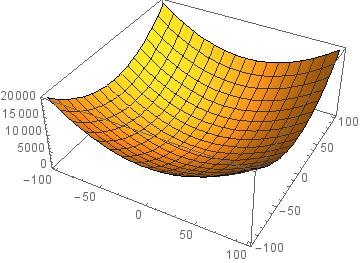
\includegraphics[scale = 0.3]{complexz2abssurface}
    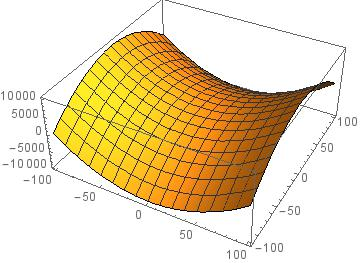
\includegraphics[scale = 0.3]{complexz2resurface}
    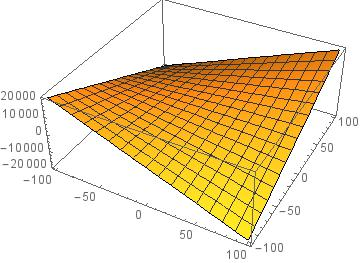
\includegraphics[scale = 0.3]{complexz2imsurface}

    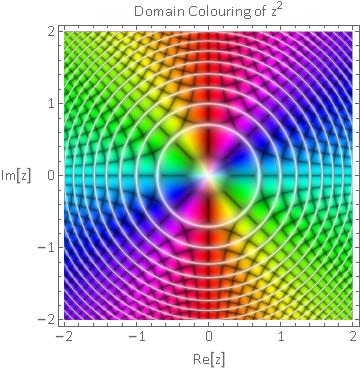
\includegraphics[scale = 0.5]{colorz2}
    \end{center}
    %
    The graph of the real part $w = \Re(z^2)$ can be written as $w = \Re(z)^2 - \Im(z)^2$. This is a hyperbololic paraboloid, as is the imaginary part can be written $w = 2\Re(z)\Im(z)$, with level curves
    %
    \[ \Im(z) = \frac{w}{2 \Re(z)} \]
    %
    Graphs of the three component functions are shown above.
\end{example}

\section{Holomorphicity}
We would like to describe what it means for a function $f$ to be a complex differentiable function at a point $z_0$. In the real case, this would hold true if there was a real linear function $\Lambda: \mathbf{C} \to \mathbf{C}$ for which
%
\[ f(z_0 + z) = f(z_0) + \Lambda z + o(z) \]
%
If $\Lambda$ is complex linear, then there is a unique $w \in \mathbf{C}$ for which $\Lambda z = wz$. In this form, we may easily extend differentiability to the complex case.

\begin{definition}
    A function $f$ is {\bf complex differentiable} at a point $z_0$ if there is $w \in \mathbf{C}$ for which
    %
    \[ f(z_0 + z) = f(z_0) + wz + o(z) \]
    %
    or if
    %
    \[ \lim_{z \to 0} \frac{f(z_0 + z) - f(z_0)}{z} = w \]
    %
    We call $w$ the derivative of $f$ at $z_0$, and write $w = f'(z_0)$. A function on an open set is {\bf holomorphic} if it is differentiable at every point in its domain, or in general, if it may be extended to be differentiable on an open set containing its domain. A function is {\bf entire} if it is holomorphic on $\mathbf{C}$. The set of all holomorphic functions defined on a set $D$ is denoted $C^\omega(D)$.
\end{definition}

Locally, a holomorphic function is just complex multiplication, characterized by a translation and a homothety.

\begin{example}
    The function $f(z) = z$ is entire, with $f'(z) = 1$. In general, a polynomial
    %
    \[ f(z) = \sum_{k = 0}^n a_k z^k \]
    %
    is entire with derivative
    %
    \[ f'(z) = \sum_{k = 1}^n k a_k z^{k-1} = \sum_{k = 0}^{n-1} (k + 1) a_{k+1} z^k \]
    %
    In general, every rational function is holomorphic on the set upon which it is defined (where the denominator does not have a zero).
\end{example}

The standard rules of calculus apply in the complex plane, and the proofs go through with little to no modification. For instance,
%
\[ (f + g)'(z_0) = f'(z_0) + g'(z_0)\ \ \ \ \ (fg)'(z_0) = f(z_0)g'(z_0) + f'(z_0)g(z_0) \]
%
\[ \left(\frac{f}{g}\right)'(z_0) = \frac{f'(z_0)g(z_0) - f(z_0)g'(z_0)}{g^2(z_0)}\ \ \ \ \ (f \circ g)'(z_0) = (f' \circ g)(z_0) g'(z_0) \]
%
We leave these to the reader to verify, or take for granted.

Though it may seem as a simple modification for real differentiability, we shall see that holomorphic functions exhibit much more marvelous and complex phenomena.

\begin{example}
    The function $f(z) = \overline{z}$ is not holomorphic. We express the limit as
    %
    \[ \lim_{a + bi \to 0} \frac{f(z_0 + (a + bi)) - f(z_0)}{a + bi} = \lim_{a + bi \to 0} \frac{a - bi}{a + bi} \]
    %
    If this limit were to exist, then surely we could calculate it by approximating from the imaginary axis
    %
    \[ \lim_{b \to 0} \frac{-bi}{bi} = -1 \]
    %
    And also from the real axis
    %
    \[ \lim_{a \to 0} \frac{a}{a} = 1 \]
    %
    But these values are not equal, so the limit does not exist, even though the function is $C^\infty$ (in fact, more strongly, just a linear function).
\end{example}



\section{Complex Manifold Theory}

The study of differentiable manifolds generalizes calculus to spaces which are locally linear. In this section we attempt to find a complex theory of manifolds, which in the one dimensional case are known as {\bf Riemann surfaces}. Certainly, these should be 2-dimensional manifolds, with additional structure which enables us to consider holomorphic functions. On any manifold, we introduce a $C^\infty$ structure, which is an atlas of local embeddings $x:U \to \mathbf{R}$, such that if $y: V \to \mathbf{R}$ is any other embedding, $x \circ y^{-1}$ is $C^\infty$ where defined. Similarily, we introduce an atlas on complex manifolds to be a cover of the space by homeomorphisms $(x,U)$ and $(y,V)$ such that $x \circ y^{-1}$ is holomorphic where defined.

Now given a Riemann surface $M$, we may introduce a complex vector space structure to the tangent space $T_p M$. Recall that if $V$ is an $\mathbf{R}$ vector space, and $J: V \to V$ is a linear map such that $J^2 = -1$, then we may define a complex vector space structure to $V$ by defining $(a + bi)v = a + bJv$, so that a complex vector space is just a real vector space with a fixed `90 degree rotation'. We define a family of linear maps $J_p: T_p M \to T_p M$ at each point by use of the holomorphic coordinates. If $(x,U)$ is a chart at $p$, then we may write each tangent vector $v$ at $p$ in the coordinates of $x$ with a unique $z \in \mathbf{C}$, by the correspondence $x_*$. We define $Jv$ in the coordinates of $x$ to be $iz$. If $y$ is another chart at $p$, then $v$ has coordinates $(y \circ x^{-1})'(x(p)) \cdot z$, and $Jv$ has coordinates $(y \circ x^{-1})'(x(p))(iz) = i(y \circ x^{-1})'(x(p)) z$. Thus $J$ is independant of the coordinate system, and so the tangent spaces are one-dimensional complex vector spaces.

A map $f: M \to N$ between Riemann surfaces is holomorphic if the map is holomorphic in every coordinate system. Since we have the tangent bundle, there is a more natural coordinate-invariant definition. Provided $f$ is differentiable (which it must be if it is holomorphic), $f$ induces a map $f_*: TM \to TN$. $f$ is holomorphic if and only if $f_*$ is complex-linear at each point. Complex manifolds are manifolds where we have `local rotations' at each point, are the holomorphic functions are those which preserve local rotations.

\begin{example}
    The fundamental example of a Riemann surface is the Riemann sphere $\mathbf{C}^\infty = \mathbf{C} \cup \{ \infty \}$, whose topology is defined to be the compactification of $\mathbf{C}$. The subsets $\mathbf{C}$ and $\mathbf{C}^\infty - \{ 0 \}$ both have homeomorphisms onto $\mathbf{C}$, the first by the identity map, and the second by the map $z \mapsto 1/z$. The maps are compatible since $1/z$ is holomorphic for $z \neq 0$ on $\mathbf{C}$. A function $f: \mathbf{C}^\infty \to \mathbf{C}$ is holomorphic if and only if $f(z)$, and $f(1/z)$ are holomorphic. Life is more fun if we consider holomorphic functions from $\mathbf{C}$ to $\mathbf{C}^\infty$, which are meromorphic functions, and holomorphic functions from $\mathbf{C}^\infty$ to $\mathbf{C}^\infty$, which are meromorphic functions meromorphic at $\infty$.
\end{example}

Fundamentally, the `$J$' map is what defines the holomorphic properties of a $2$-manifold. If a given bundle map $J:TM \to TM$ is given such that $J^2 = -1$, then this map defines a complex linear structure on the tangent spaces, and we define $f: M \to N$ to be holomorphic if the corresponding map $f_*$ is complex linear at each point. A holomorphic atlas on $M$ may then be define to be the set of all `holomorphic charts', for if $(x,U)$ and $(y,V)$ are holomorphic charts, then $x \circ y^{-1}$ is holomorphic, for it is certainly differentiable, and the derivative is complex linear. Thus as long as $J$ is `consistant', in the sense that there exist enough holomorphic charts to cover the manifold, then $J$ is a perfectly reasonable way to define a complex structure on a $2$-manifold. In fact, $J$ is what we call a {\bf almost complex structure} on the manifold, for it is almost all we need to define holomorphic functions.

Even if we forget the tangent space $T_p M$, we may still reconstruct it from a holomorphic atlas by considering derivations. Recall that a $p$-derivation is a complex-valued function $\Lambda$ such that for any two functions $f,g \in C^\infty(M,\mathbf{C})$,
%
\[ \Lambda (fg) = f(p) \Lambda g + g(p) \Lambda f \]
%
By induction, provided $f_i(p) \neq 0$ for any $p$,
%
\[ \Lambda \left(\prod_{i = 1}^n f_i \right) = \prod_{i = 1}^n f_i(p) \left[\sum_{i = 1}^n \frac{\Lambda f_i}{f_i(p)}\right] \]
%
If we define the partial differential operators
%
\[ \deriv{f}{x}{p} = \left.\frac{\partial \Re f}{\partial x}\right|_p + i \left.\frac{\partial \Im f}{\partial x}\right|_p\ \ \ \ \ \left.\frac{\partial f}{\partial y}\right|_p = \left.\frac{\partial \Re f}{\partial y}\right|_p + \left.\frac{\partial \Im f}{\partial y}\right|_p \]
%
Then these operators are easily shown to be contained in $T_p \mathbf{C}$. As in the real case, we shall show these operators span over the complex linear space $T_p \mathbf{C}$, that is, every linear operator in $T_p \mathbf{C}$ can be written as a complex combination of the two operators. The proof is not too different from the real case. In the sequel, we shall let $\Lambda$ stand for an arbitrary $p$-derivation.

\begin{lemma}
    If $c$ is a constant function $c: w \to c$, for $c \in \mathbf{C}$, then $\Lambda c = 0$.
\end{lemma}
\begin{proof}
    Consider the constant $1$ function. Then $1 = 1 \cdotp 1$, so
    %
    \[ \Lambda 1 = \Lambda (1 \cdotp 1) = \Lambda 1 + \Lambda 1 \]
    %
    Hence $\Lambda 1 = 0$. Now $\Lambda c = c \Lambda 1 = c \cdotp 0 = 0$.
\end{proof}

\begin{lemma}
    If $f$ and $g$ are equal in a neighbourhood of $p$, then $\Lambda f = \Lambda g$.
\end{lemma}
\begin{proof}
    If $f$ and $g$ are as above, then $f - g$ is constantly zero in a neighbourhood $U$ of $p$ (which we may assume to be bounded). Consider a function $\Psi$ which has value 1 on a closed neighbourhood $\overline{V} \subset U$, and which vanishes outside of $U$. Then $(f - g) \Psi = 0$, so
    %
    \[ 0 = \Lambda 0 = \Lambda (f - g) \Psi = (f - g)(p) \Lambda \Psi + \Psi(p) \Lambda (f - g) = \Lambda f - \Lambda g \]
    %
    And we have shown $\Lambda f = \Lambda g$.
\end{proof}

It is for this reason that Grothendieck thought of the tangent space as defined on the {\it sheaf} generated by the $C^\infty$ functions, that is, the equivalence classes of functions locally equal around $p$.

\begin{corollary}
    $T_p U$ is isomorphic to $T_p \mathbf{C}$, for any open subset $U$ of $\mathbf{C}$.
\end{corollary}

The following is a trivial consequence of the property of a derivation.

\begin{lemma}
    If $f(p) = g(p) = 0$, then $\Lambda (fg) = 0$.
\end{lemma}

Now for the big theorem.

\begin{theorem}
    Any linear derivation $\Lambda$ can be written as the complex combination of the partial differential operators defined above.
\end{theorem}
\begin{proof}
    Consider any $f \in C^\infty \mathbf{C}$. By appealing to Taylor's theorem in the real case, one may write
    %
    \begin{align*} f(z) &= f(p) + \left.\frac{\partial f}{\partial x}\right|_p (\Re z - \Re p) + i \left. \frac{\partial f}{\partial y} \right|_p (\Im z - \Im p) + \text{Second Order Terms}...
    \end{align*}
    %
    Then
    %
    \begin{align*}
        \Lambda f &= \Lambda f(p) + \left.\frac{\partial f}{\partial x}\right|_p \Lambda(\Re z - \Re p) + i \left. \frac{\partial f}{\partial y} \right|_p \Lambda(\Im z - \Im p) + \Lambda(\text{second order terms})\\
        &= 0 + \left.\frac{\partial f}{\partial x}\right|_p \Lambda (\Re z) + i \left. \frac{\partial f}{\partial y} \right|_p \Lambda(\Im z) + 0
    \end{align*}
    %
    Considering all $f$, we conclude
    %
    \[ \Lambda = \left.\frac{\partial}{\partial x}\right|_p \Lambda (\Re z) + i \left. \frac{\partial}{\partial y} \right|_p \Lambda(\Im z) \]
    %
    And our proof is complete, any such complex combination of the form
    %
    \[ z \left.\frac{\partial}{\partial x}\right|_p + w \left. \frac{\partial}{\partial y} \right|_p \]
    %
    Is a $p$-derivation, and any $p$-derivation can be written uniquely in this form.
\end{proof}

As with a tangent space, we can consider the cotangent space $T_p^* \mathbf{C}$, the dual space of $T_p \mathbf{C}$. Given any smooth $f: \mathbf{C} \to \mathbf{C}$, we may define $df_p \in T_p^*$ by the equation
%
\[ df_p (v) = v(f) \]
%
We may put these maps together to form a map $df$ on all of $T^* \mathbf{C}$. Appealing to the theorem above, we may write any $\omega \in T_p^* \mathbf{C}$ as $z\ dx_p + w\ dy_p$. 
%
We have
%
\[ df = \frac{\partial f}{\partial x} dx + \frac{\partial f}{\partial y} dy \]

The most intriguing part of this construction occurs when we examine analytic functions. In classic notation, define $z$ to be the identity map on $\mathbf{C}$. Then $z$ is trivially smooth, and so we may consider $dz = dx + i dy$. Define $\overline{z} : w \to \overline{w}$. Then $d\overline{z} = dx - i dy$. These equations are linearly independant, and thus span the cotangent space at each point. Thus any $w \in T_p^* \mathbf{C}$ may be written
%
\[ \alpha dz + \beta d\overline{z} \]
%
In particular, this holds for any $df$. We define the coefficients
%
\[ \left.\frac{\partial f}{\partial z}\right|_p \ \ \ \ \ \left.\frac{\partial f}{\partial \overline{z}}\right|_p \]
%
by the equation
%
\[ df = \left.\frac{\partial f}{\partial z}\right|_p dz + \left.\frac{\partial f}{\partial \overline{z}}\right|_p d \overline{z} \]
%
Since
%
\[ \alpha dz + \beta d\overline{z} = (\alpha + \beta) dx + i(\alpha - \beta) dy \]
%
We obtain the equalities
%
\[ \frac{\partial f}{\partial z} + \frac{\partial f}{\partial \overline{z}} = \frac{\partial f}{\partial x}\ \ \ \ \ \frac{\partial f}{\partial z} - \frac{\partial f}{\partial \overline{z}} = -i \frac{\partial f}{\partial y} \]
%
Reordering these equations, we determine that
%
\[ \frac{\partial f}{\partial z} = \frac{1}{2} \left( \frac{\partial f}{\partial x} - i \frac{\partial f}{\partial y} \right)\ \ \ \ \ \frac{\partial f}{\partial \overline{z}} = \frac{1}{2} \left( \frac{\partial f}{\partial x} + i \frac{\partial f}{\partial y} \right) \]
%
The conjugate map $T: z \mapsto \overline{z}$ is a real linear map which is not complex linear. If $U$ is the identity map, then every real linear map $S: \mathbf{C} \to \mathbf{C}$ may be uniquely written as $zT + wI$, with $z,w \in \mathbf{C}$. To see this, we calculate $T$, $iT$, $I$, and $iI$ in matrix notation
%
\[ T = \begin{pmatrix} 1 & 0 \\ 0 & -1 \end{pmatrix} \ \ \ \ \ \ \ iT = \begin{pmatrix} 0 & -1 \\ 1 & 0 \end{pmatrix} \begin{pmatrix} 1 & 0 \\ 0 & -1 \end{pmatrix} = \begin{pmatrix} 0 & 1 \\ 1 & 0 \end{pmatrix} \]
%
\[ I = \begin{pmatrix} 1 & 0 \\ 0 & 1 \end{pmatrix}\ \ \ \ \ \ \ \ iI = \begin{pmatrix} 0 & -1 \\ 1 & 0 \end{pmatrix} \]
%
and then find the four matrices are linearly independant over $\mathbf{R}$, hence a spanning set. Thus our discussion is a simple generalization of this fact to arbitrary differentiable maps, since $dz$ is equal to the identity matrix $I$, and $d \overline{z}$ is equal to $T$, on each fibre $T_p \mathbf{C}$.




\section{The Cauchy-Riemann Equations}

We emphasize that to be complex differentiable, a function must be approximated locally by a {\it complex linear function}. In two dimensions, the only functions of this type are of the form $\Lambda z = wz$. Let us calculate what the matrix representation of $\Lambda$ is with respect to the basis $\mathcal{B} = (1, i)$ in $\mathbf{C}$. If $w = a + bi$, then
%
\[ [\Lambda]_{\mathcal{B}} = \begin{pmatrix} a & b \\ -b & a \end{pmatrix} \]
%
Geometrically, $\Lambda$ is just a homothety, a rotation and a dilation (stretching). Since $\Lambda$ is well defined at $z_0$, we may take partial derivatives, and conclude
%
\[ \deriv{\Re f}{x}{z_0} = a = \deriv{\Im f}{y}{z_0}\ \ \ \ \ \deriv{\Im f}{x}{z_0} = b = -\deriv{\Re f}{y}{z_0} \]
%
Putting these equations together, we may write
%
\[ \deriv{f}{x}{z_0} = -i \deriv{f}{y}{z_0} \]
%
Where we define the complex partial derivative linear on each factor. Conversely, if this equation holds, and $f$ is continuously differentiable, then a complex linear $\Lambda$ exists at $z_0$. We have something of practical importance for determining if a function is holomorphic.

\begin{theorem}
    A function $f$ satisfies the {\bf Cauchy-Riemann equations} at a point $z_0$ if
    %
    \[ \deriv{f}{x}{z_0} = -i \deriv{f}{y}{z_0} \]
    %
    If $f$ is complex differentiable at $z_0$, then $f$ satisfies the Cauchy-Riemann equations. Conversely, if $f$ is $C^1$ and satisfies the Cauchy-Riemann equations at $z_0$, then $f$ is complex differentiable at $z_0$.
\end{theorem}

In the language of the complex tangent space, the Cauchy-Riemann equation states exactly that
%
\[ \frac{\partial f}{\partial \overline{z}} = 0 \]
%
Now as with $C^\infty \mathbf{C}$, we may consider all derivations on $C^\omega \mathbf{C}$, to determine the analytic tangent space $T^\omega \mathbf{C}$. Surely, we may restrict the functions in $C^\infty \mathbf{C}$ to $C^\omega \mathbf{C}$, but this does not imply the sets are the same, for two functions which differ originally may be equal when restricted to a smaller set. Since the inclusion $i:C^\omega \mathbf{C} \to C^\infty \mathbf{C}$ is injective, We obtain a surjective bundle map $i^*: T \mathbf{C} \to T^\omega \mathbf{C}$. The kernel of this map (when restricted to the tangent space) is precisely the linear operators of the form
%
\[ \beta \frac{\partial}{\partial \overline{z}} \]
%
Therefore all derivations on $C^\omega \mathbf{C}$ can be written as
%
\[ w \frac{\partial}{\partial z} \]
%
And so this space is one dimensional.

When analyzing the analytic case, we often write the operator as
%
\[ \frac{df}{dz} \]
%
To mimic the 1-dimensional real case. For any analytic function $f$, we have
%
\[ df = \frac{df}{dz} dz \]
%
Most of the real theorems on the tangent space apply to the complex case due to the extension of definitions by linearity. In particular, Stoke's theorem also holds, so if $\Delta$ is an open set in $\mathbf{C}$ whose boundary is a one-manifold, then
%
\[ \int_{\partial \Delta} f\ dz = \int_\Delta \frac{df}{dz}\ dz \wedge dz = \int_\Delta 0 = 0 \]
%
We may consider complex differentiable forms, for instance, and if $\Delta$ is a contractible, open set of $\mathbf{C}$, on which $d \omega = 0$, then $\omega = df$ for some analytic function $f$.



\section{Power Series}

Polynomials are the simplest examples of holomorphic functions. Our next family of holomorphic functions will be obtained by taking limits of polynomials. In fact, we will soon show that this family contains all holomorphic functions.

\begin{definition}
    A {\bf formal power series} around a point $z_0$ is an `infinite dimensional polynomial', a sequence written in the form
    %
    \[ \sum_{k = 0}^\infty c_k (z - z_0)^k \]
    %
    The $c_k$ are known as the coefficients of the series. We may evaluate a power series to obtain a function $f$, defined as
    %
    \[ f(z) = \sum_{k = 0}^\infty a_k (z - z_0)^k \]
    %
    whose domain is the set where the series converges. A function $f$ can be {\bf expanded in a power series} at a point $z_0$ if we may write $f$ as a power series locally around $z_0$. An {\bf analytic} function is a function which can be locally expanded as a power series at every point in its domain.
\end{definition}

Standard tricks from real power series come into play here, and the proofs go unedited. The most useful is the root test, or Cauchy-Hadamard theorem, which states that, if we define
%
\[ 1/R = \limsup_{n \to \infty} |c_n|^{1/n} \]
%
Then the power series $f$ converges for $|z - z_0| < R$, and diverges for $|z - z_0| > R$. It may sometimes be easier to apply the ratio test. If the limit
%
\[ L^{-1} = \lim_{n \to \infty} \left| \frac{c_{n+1}}{c_n} \right| \]
%
exists, then $f$ converges for $|z - z_0| < L$, and diverges for $|z - z_0| > L$. These statements do not say anything about what happens on the boundary, when $|z - z_0|$ is equal to $R$ or $L$. If $g$ 

If $g$ can also be expanded as a power series at $z_0$,
%
\[ g(z) = \sum_{k = 0}^\infty a_k (z - z_0)^k \]
%
Then $(fg)$ can also be expanded at the point, and we have the product formula
%
\[ (fg)(z) = \sum_{m = 0}^\infty \left( \sum_{k = 0}^m a^kc^{m-k} \right) (z - z_0)^k \]
%
The quotient of two power series is also a power series, but we are not able to discuss this with our current knowledge. Thus the set of all analytic functions has a nice algebraic structure.

\section{The Exponential, and Series Differentiation}

The most important power series, and perhaps the most important function in mathematics, is the exponential function, defined at all points in the complex plane by the formula
%
\[ e^z = \exp(z) = \sum_{k = 0}^\infty \frac{z^k}{k!} \]
%
The product formula above shows that
%
\begin{align*}
    \exp(z + w) &= \sum_{k = 0}^\infty \frac{(z + w)^k}{k!} = \sum_{k = 0}^\infty \sum_{j = 0}^k \binom{k}{j} \frac{z^j w^{k-j}}{k!}\\
    &= \sum_{k = 0}^\infty \sum_{j = 0}^k \frac{z^j}{j!} \frac{w^{k-j}}{(k - j)!} = \exp(z) \exp(w)
\end{align*}
%
Which gives us the multiplicative property of the function.

Calculus tells us that the derivative of the exponential function is the exponential function itself. If there is any justice in the world, this idea should extend to the complex case. We can calculate
%
\[ \exp'(z) = \sum_{k = 0}^\infty \left( \frac{z^k}{k!} \right)' = \sum_{k = 1}^\infty \frac{z^{k-1}}{(k-1)!} = \sum_{k = 0}^\infty \frac{z^k}{k!} = \exp(z) \]
%
But how do we know that the derivative of the power series can be obtained by differentiating each term in the series?

\begin{theorem}
    Let $f(z) = \sum_{k = 0}^\infty c_k z^k$ be a power series, convergent inside a disk $D$. Then $f$ is holomorphic in $D$, and $f'(z) = \sum_{k = 1}^\infty k c_k z^{k-1}$.
\end{theorem}
\begin{proof}
    The fact that the power series defining $f'$ converges in $D$ follows from the Hadamard formula. Now let us verify that this series, which defines a function $g$, approaches the derivative of $f$. Define $S_n$ to be the finite polynomial of degree $n$ defined by $f$, $S_n(z) = \sum_{k = 0}^n c_k z^k$. Let $E_n$ denote the error term, $E_n(z) = \sum_{k = n+1}^\infty c_k z^k$. Then $S_n'(z) = \sum_{k = 1}^n k c_k z^{k-1}$, and
    %
    \[ \frac{f(z + w) - f(z)}{w} = \left[ \frac{S_n(z + w) - S_n(z)}{w} - S_n'(z) \right] + \left[ \frac{E_n(z + w) - E_n(z)}{w} \right] + S_n'(z) \]
    %
    The first term converges to zero for small enough $w$. The third term converges to $g(z)$ as $n \to \infty$. The only tricky component is the second term. Since $a^n - b^n = (a - b)(a^{n-1} + a^{n-2}b + \dots + ab^{n-2} + b^{n-1})$. If we choose $|z|, |z + w| < r - \varepsilon$, then
    %
    \begin{align*}
        \left| \frac{E_n(z + w) - E_n(z)}{w} \right| &= \left| \sum_{k = n + 1}^\infty c_k \frac{(z + w)^k - z^k}{w} \right| \leq \sum_{k = n + 1}^\infty k |c_k| (r - \varepsilon)^{n-1}
    \end{align*}
    %
    The right side is a convergent power series, and hence as $n \to \infty$, the term converges to zero. By picking $n$ large enough, and $|z - w|$ small enough, the value can be made as close to $g$ as possible.
\end{proof}

\begin{corollary}
    A function $f(z) = \sum_{i = 0}^\infty c_i z^i$ expandable in a power series about a point has holomorphic derivatives $f', f'', f^{(3)}, \dots$ around the point, which are also expandable in a power series
    %
    \[ f^{(n)} = \sum_{k = n}^\infty \frac{k!}{(k - n)!} c_k z^{k-n} \]
\end{corollary}

\begin{corollary}
    Every analytic function is holomorphic
\end{corollary}

We shall later prove that every holomorphic function is analytic. First, let us examine some useful properties of the exponential. Most sensationally, we shall verify Euler's formula
%
\[ e^{i \pi} = 1 \]
%
This fact depends on the fact that the complex exponential function is much more robust than 



\chapter{Geometric Function Theory}

An intuitive way to visualize analytic functions is how they act on the geometry of the complex plane. The Riemann school believes that this should be the primary way of understanding these maps, giving us interesting geometric results. Here we introduce conformal maps, and pave the way to Riemann's classical mapping theorem.

The study of geometry was fundamentally changed by Felix Klein's Erlangen program. To rationalize the emergence of the paradoxical non-euclidean geometries, The fundamental thesis of the program is that a study of the invariants of space under actions from a certain group. Klein's Euclidean geometry studies invariants of the plane invariant under similarity transformations, which preserve angles and proportions, collected into the Euclidean group $E(2)$. Projective geometry studies invariants of the sphere under transformations which preserve the incidence of straight lines, collected into the projective group $P(2)$. Of course, one may perturb these groups to obtain more interesting results. For instance, to study properties of space which remain after oriented similarity, we weaken our actions to the special euclidean group $SE(2)$, a subgroup of $E(2)$.

Geometrically, the set of all {\bf biholomorphic functions} (holomorphic maps with a holomorphic inverse) forms a group.

After studying all these analytic functions, it is of course, of interest to determine the properties of the plane which remain invariant under the actions of bijective analytic functions, which form a group.

Let us pretend we have never seen the definition of an analytic function. In fact, forget we have ever invented complex numbers at all (we consider $\mathbf{C}$ as another name for the real plane $\mathbf{R}^2$). $\mathbf{C}$ is a two-dimensional surface, and therefore posseses a tangent space $T\mathbf{C}$, which naturally can be considered as $\mathbf{C}^2$ -- tangent vectors in this space will be denoted as $v_p$, the vector $v$ at the point $p$. $T\mathbf{C}$ is also a Riemannian manifold, since we have a natural inner product on the tangent vectors at each point on the plane, defined by
%
\[ \langle v_p, w_p \rangle = v_1 w_1 + v_2 w_2 = \Re[v\overline{w}] \]
%
One obtains `infinitisimal' equivalents to the structures on an inner product space. For instance, one may talk about the `infinitisimal' length of a tangent vector, defined by
%
\[ \| v_p \| = \langle v_p, v_p \rangle \]
%
More interesting to us, we are able to talk about `infinitisimal angles' at points. That is, the angle between two tangent vectors $v_p$ and and $w_p$ is the angle $\theta$ such that
%
\[ \cos(\theta) = \frac{\langle v_p, w_p \rangle}{\|v\| \|w\|} \]
%
We are now ready to discuss conformal maps, the geometric method of introducing analytic functions.

\begin{definition}
    A complex-valued differentiable map $f$ defined on an open subset of the plane is {\bf conformal} if it is oriented, and preserves infinitisimal angles. Pointwise conformality is defined similarily
\end{definition}

\begin{lemma}
    A function analytic at a point with non-zero derivative is conformal there.
\end{lemma}
\begin{proof}
    Let $f$ be analytic at $p$, with $f'(p) = z \neq 0$. The matrix representation of $f'(p)$ is
    %
    \[ \begin{pmatrix} \Re[z] & \Im[z] \\ -\Im[z] & \Re[z] \end{pmatrix} \]
    %
    Whose determinant is $\Re[z]^2 + \Im[z]^2 > 0$, hence the map is oriented at $p$. A calculation verifies that
    %
    \[ \langle f^*(v_p), f^*(w_p) \rangle = \langle zv, zw \rangle = |z|^2 \langle v, w \rangle  \]
    %
    So that, since $|zv| = |z||v|$, and $|zw| = |z||w|$,
    %
    \[ \frac{\langle zv, zw \rangle}{|zv||zw|} = \frac{|z|^2 \langle v, w \rangle }{|z|^2|v||w|} = \frac{\langle v, w \rangle}{|v||w|} \]
    %
    Thus the map is conformal.
\end{proof}

We shall show that, the differential map at any point in the plane is just a rotation and scaling. For each unit tangent vector $e^{i\theta}$ at a point $p$, consider the differential map $f_*((e^{i\theta})_p)$.

Let us now use our knowledge of the complex plane to reintroduce an old friend. We may express the differential of a conformal map $f = u + iv$ as
%
\[ f^*(v_p) = \]

Consider the action of a conformal map $f$ on the unit tangent vectors $(e_1)_p$ and $(e_2)_p$
%
\[ f^*((e_1)_p) = Df(p)(e_1) = \deriv{f^1}{x}{p} \deriv{}{x}{f(p)} + \deriv{f^2}{x}{p} \deriv{}{y}{f(p)} \]
%
\[ f^*((e_2)_p) = Df(p)(e_2) = \deriv{f^1}{y}{p} \deriv{}{x}{f(p)} + \deriv{f^2}{y}{p} \deriv{}{y}{f(p)} \]
%
Since $f$ is conformal, these vectors must be at right angles, and $(f^*(1_p), f^*(i_p))$ must be an oriented basis. In two dimensions, the only vectors orthogonal to a vector $v = (a,b)$ are scalar multiples of the vector $w = (-b,a)$. Since $(v, \lambda w)$ must be oriented, we must have $\lambda (a^2 + b^2) > 0$, hence $\lambda > 0$. Taken in the case of our conformally mapped tangent vectors, we must have some $\lambda > 0$ for which,
%
\[ f^*((e_2)_p) = \lambda \left( -\deriv{f^2}{x}{p} \deriv{}{x}{f(p)} + \deriv{f^1}{x}{p} \deriv{}{y}{f(p)} \right) \]
%
Equating our two values of $f^*((e_2)_p)$, we see that
%
\[ \deriv{f^1}{y}{p} = - \lambda \deriv{f^2}{x}{p}\ \ \ \ \ \deriv{f^2}{y}{p} = \lambda \deriv{f^1}{x}{p} \]

\begin{thebibliography}{10}
    \bibitem{intro} Michael Spivak,
    \emph{A Concise Introduction to Differential Geometry: Vol. One}

    \bibitem{halm} Paul Halmos,
    \emph{Naive Set Theory}

    \bibitem{wiki} Wikipedia,
    \emph{Lie Groups}
\end{thebibliography}

\end{document}